\chapter{The CMS Experiment and the LHC}
\label{ch:cms}
The Compact Muon Solenoid (CMS) detector is a multi-purpose detector
conceived to study proton-proton (and lead-lead) collisions produced
by the Large Hadron Collider (LHC) at CERN~\cite{Adolphi:2008zzk}.
The central feature of the CMS detector is a
superconducting solenoid of 6\unit{m} internal diameter, providing a
magnetic field of 3.8\unit{T}. Within the superconducting solenoid
volume are a silicon pixel and a silicon strip tracker, a
lead-tungstate crystal electromagnetic calorimeter, and a
brass/scintillator hadron calorimeter, each composed of a barrel and
two endcap sections. Muons are measured in gas-ionization detectors
embedded in the magnet steel flux-return yoke outside the
solenoid. Extensive forward calorimetry complements the coverage
provided by the barrel and endcap detectors. Jets and leptons are
reconstructed within the pseudorapidity region $\abs{\eta}<3$, covered by the
electromagnetic and hadron calorimeters. Muons are reconstructed with
$\abs{\eta}<2.4$. Events are selected by a
two-level trigger system. The first level (L1) is based on a hardware
filter, followed by a software-based high level trigger (HLT). 
%A more detailed description of the CMS detector, together with a definition
%of the coordinate system used and the relevant kinematic variables,
%can be found in Ref.~\cite{Adolphi:2008zzk}.


\section{Large Hadron Collider}
The Large Hadron Collider (LHC) is a 27\unit{km} two-ring superconducting
proton accelerator and collider located at CERN, spanning the border between
France and Switzerland.  At design specifications, the LHC will collide
protons at a center-of-mass energy of 14\TeV and instantaneous
luminosity $10^{34} \unit{cm}^{-2} \unit{s}^{-1}$.
\begin{table*}
\centering
 \caption{Comparison between LHC design parameters and achieved
   parameters in 2012 and 2015.
 \label{tab:LHCparameters}}
\resizebox{\textwidth}{!}{
\begin{tabular}{|l|c|c|c|c|}
\hline 
Parameter & Unit & \textbf{Design} & \textbf{Acheived (2012)} & \textbf{Acheived (2015)} \\\hline
\multicolumn{5}{|c|}{\textbf{Beam Data}}\\\hline
Proton energy & [GeV] & 7000 & 4000 & 6500 \\\hline
Relativistic gamma factor $\gamma_r$ & & 7461 & 4263 & 6928 \\\hline
Number of particles per bunch $N_b$ & & $1.15\times10^{11}$ &
                                                        $1.6-1.7\times10^{11}$ & $1.15\times10^{11}$ \\\hline
Number of bunches $n_b$ & & 2808 & 1374 & 2244 \\\hline
Bunch spacing & [ns] & 25 & 50 & 25 \\\hline
%Longitudinal emittance ($4\sigma$) & [eV s] & 2.5 & & \\\hline
Transverse normalized emittance $\varepsilon_n$& [$\mu$m rad] & 3.75
                                   &2.5& $\geq2.7$\\\hline
Circulating beam current & [A] & 0.582 & 0.369&\\\hline
Stored energy per beam & [MJ] & 362 & 140 &\\\hline
\multicolumn{5}{|c|}{\textbf{Peak Luminosity Related Data}}\\\hline
$\beta^{\ast}$ at IP1 and IP5 & [m] &0.55 & 0.6 & 0.8 \\\hline
RMS bunch length $\sigma_z$& [cm] & 7.55 & $\geq 9$ &\\\hline
RMS beam size at IP1 and IP5 $\sigma^{\ast}$ & [$\mu$m] & 16.7 & 19 &\\\hline 
Half crossing angle at IP1 and IP5 $\theta_c/2$& [$\mu$rad] & $\pm142.5$ &
                                                               $\pm145.0$ & $\pm145.0$\\\hline
Geometric luminosity reduction factor $F$ & &0.836 & &\\\hline
Peak luminosity in IP1 and IP5 & [cm$^{-1}$s$^{-1}$] &
                                                       $1.0\times10^{34}$ & $7.7\times10^{33}$ & $5.2\times10^{33}$ \\\hline
Max. mean number of events per bunch crossing& & 19 & 40 & 17 \\\hline
\end{tabular}
}
\end{table*}

The LHC is the pinnacle of the accelerator
complex at CERN, pictured in Fig.~\ref{fig:LHCComplex}.  To accelerate
protons to a beam energy of 6.5\TeV in the LHC, a chain of smaller
accelerators are needed. Starting from bottle of hydrogen gas,
electrons are stripped from the hydrogen atoms by an electric field
and the resulting protons enter the Linac 2, which accelerates the
protons to 50\MeV. Subsequently, the Proton Synchrotron Booster (PSB), Proton Synchrotron (PS), and the
Super Proton Synchrotron (SPS) accelerate the protons to 1.4\GeV, 25\GeV, and 450\GeV, respectively, before they are finally injected
into the two LHC rings as counter-rotating beams.

\begin{figure}
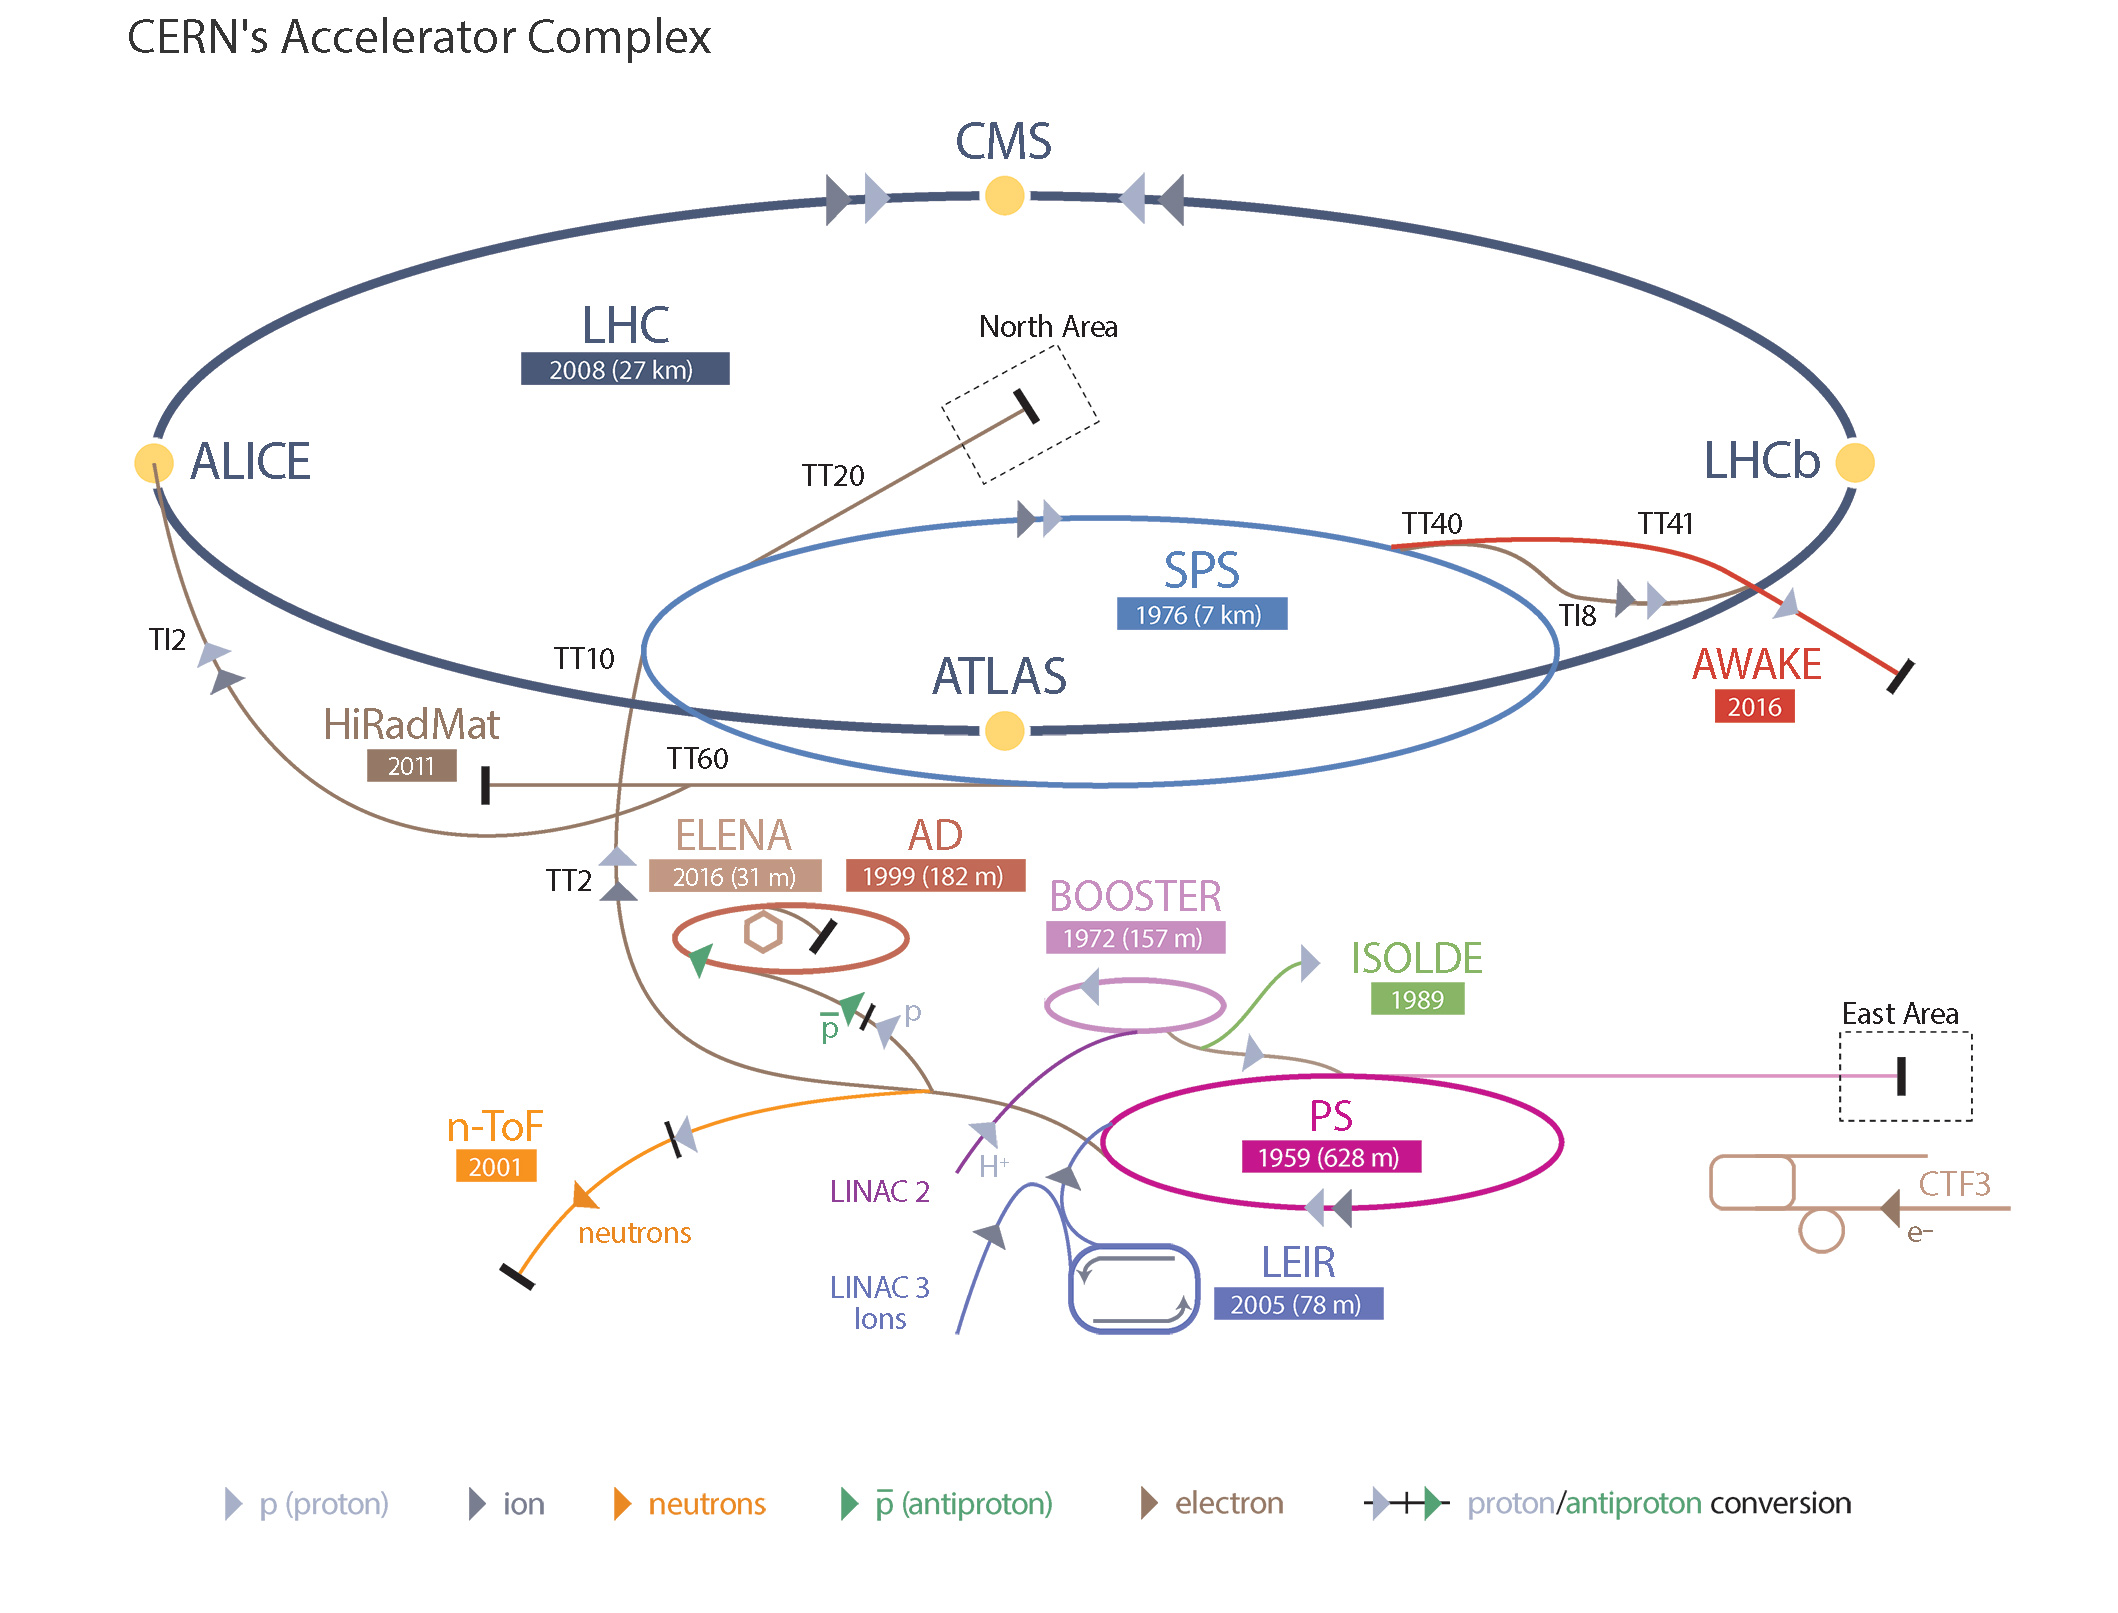
\includegraphics[width=.9\textwidth]{figs/cms/LHC_default.jpg}
\caption{CERN's accelerator complex.\label{fig:LHCComplex}}
\end{figure}

One of the main features influencing the design of the LHC is the re-use of the
existing 26.7\unit{km} tunnel from the Large Electron Positron collider (LEP), which is
comprised of eight crossing points (or arcs) and eight straight sections for
RF cavities. The tunnel in the arc sections has an internal diameter of 3.7\unit{m}. Due to the limited available space, two completely separate
proton rings would be extremely difficult to install.  magnets
would be  difficult to fit in which makes the twin-bore magnet design proposed by John
Blewett in 1971~\cite{Blewett:1068131} ideal due to its
``two-in-one'' use of the limited space. A cross-section of the main superconducting
dipole magnet is shown in \ref{fig:LHCDipole}.

\begin{figure}
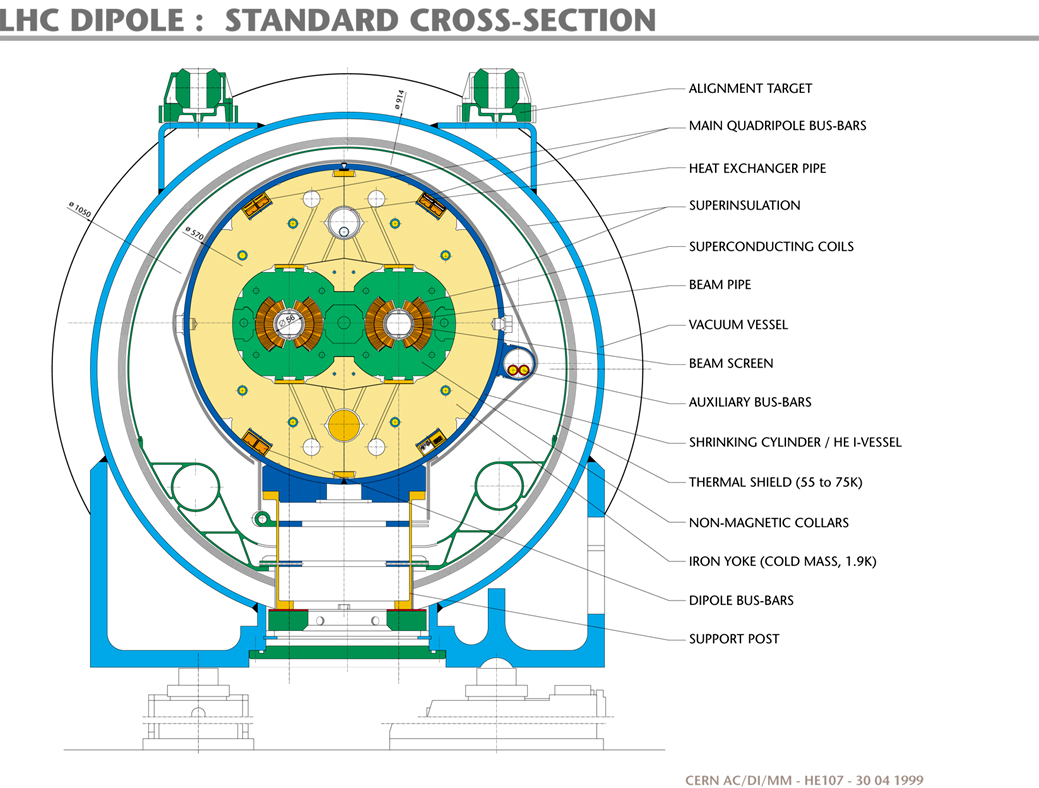
\includegraphics[width=.9\textwidth,clip=true,viewport=0 20 680 550]{figs/cms/lhc-pho-1999-172.jpg}
\caption{Cross-section of the LHC dipole magnet.\label{fig:LHCDipole}}
\end{figure}


The observed number of events $N_{\mathrm{exp}}$ is the product of the cross
section of interest $\sigma_{\mathrm{exp}}$ and the time integral of
the instantaneous luminosity,
\begin{equation}
N_{\mathrm{exp}}  =\sigma_{\mathrm{exp}}\int \mathscr{L}(t)dt ~.
\end{equation}
The instantaneous luminosity depends on the beam parameters and
can be written for a Gaussian beam distribution as~\cite{LHCMachine}:
\begin{equation}
\mathscr{L} =
\frac{N_b^2n_bf_{\mathrm{rev}}\gamma_r}{4\pi\varepsilon_n\beta^{\ast}}F~,
\label{eqn:instlumi}
\end{equation}
where $N_b$ is the number of particles per bunch, $n_b$ the number
of bunches per beam, $f_{\mathrm{rev}}$ the revolution frequency,
$\gamma_r$ the relativistic gamma factor, $\varepsilon_n$ the
normalized transverse beam emittance, $\beta^{\ast}$ the beta function
at the collision point, and $F$ the geometric luminosity reduction
factor due to the crossing angle at the interaction point (IP):
\begin{equation}
F=\left(1+\left(\frac{\theta_c\sigma_z}{2\sigma^{\ast}}\right)^2\right)^{-1/2}~,
\label{eqn:F}
\end{equation}
where $\theta_c$ is the full crossing angle, $\sigma_z$ is the RMS
bunch length, and $\sigma^{\ast}$ is the RMS bunch size.

\section {Level-1 and High Level Trigger}

\section{Alignment and Calibration}


\begin{figure}
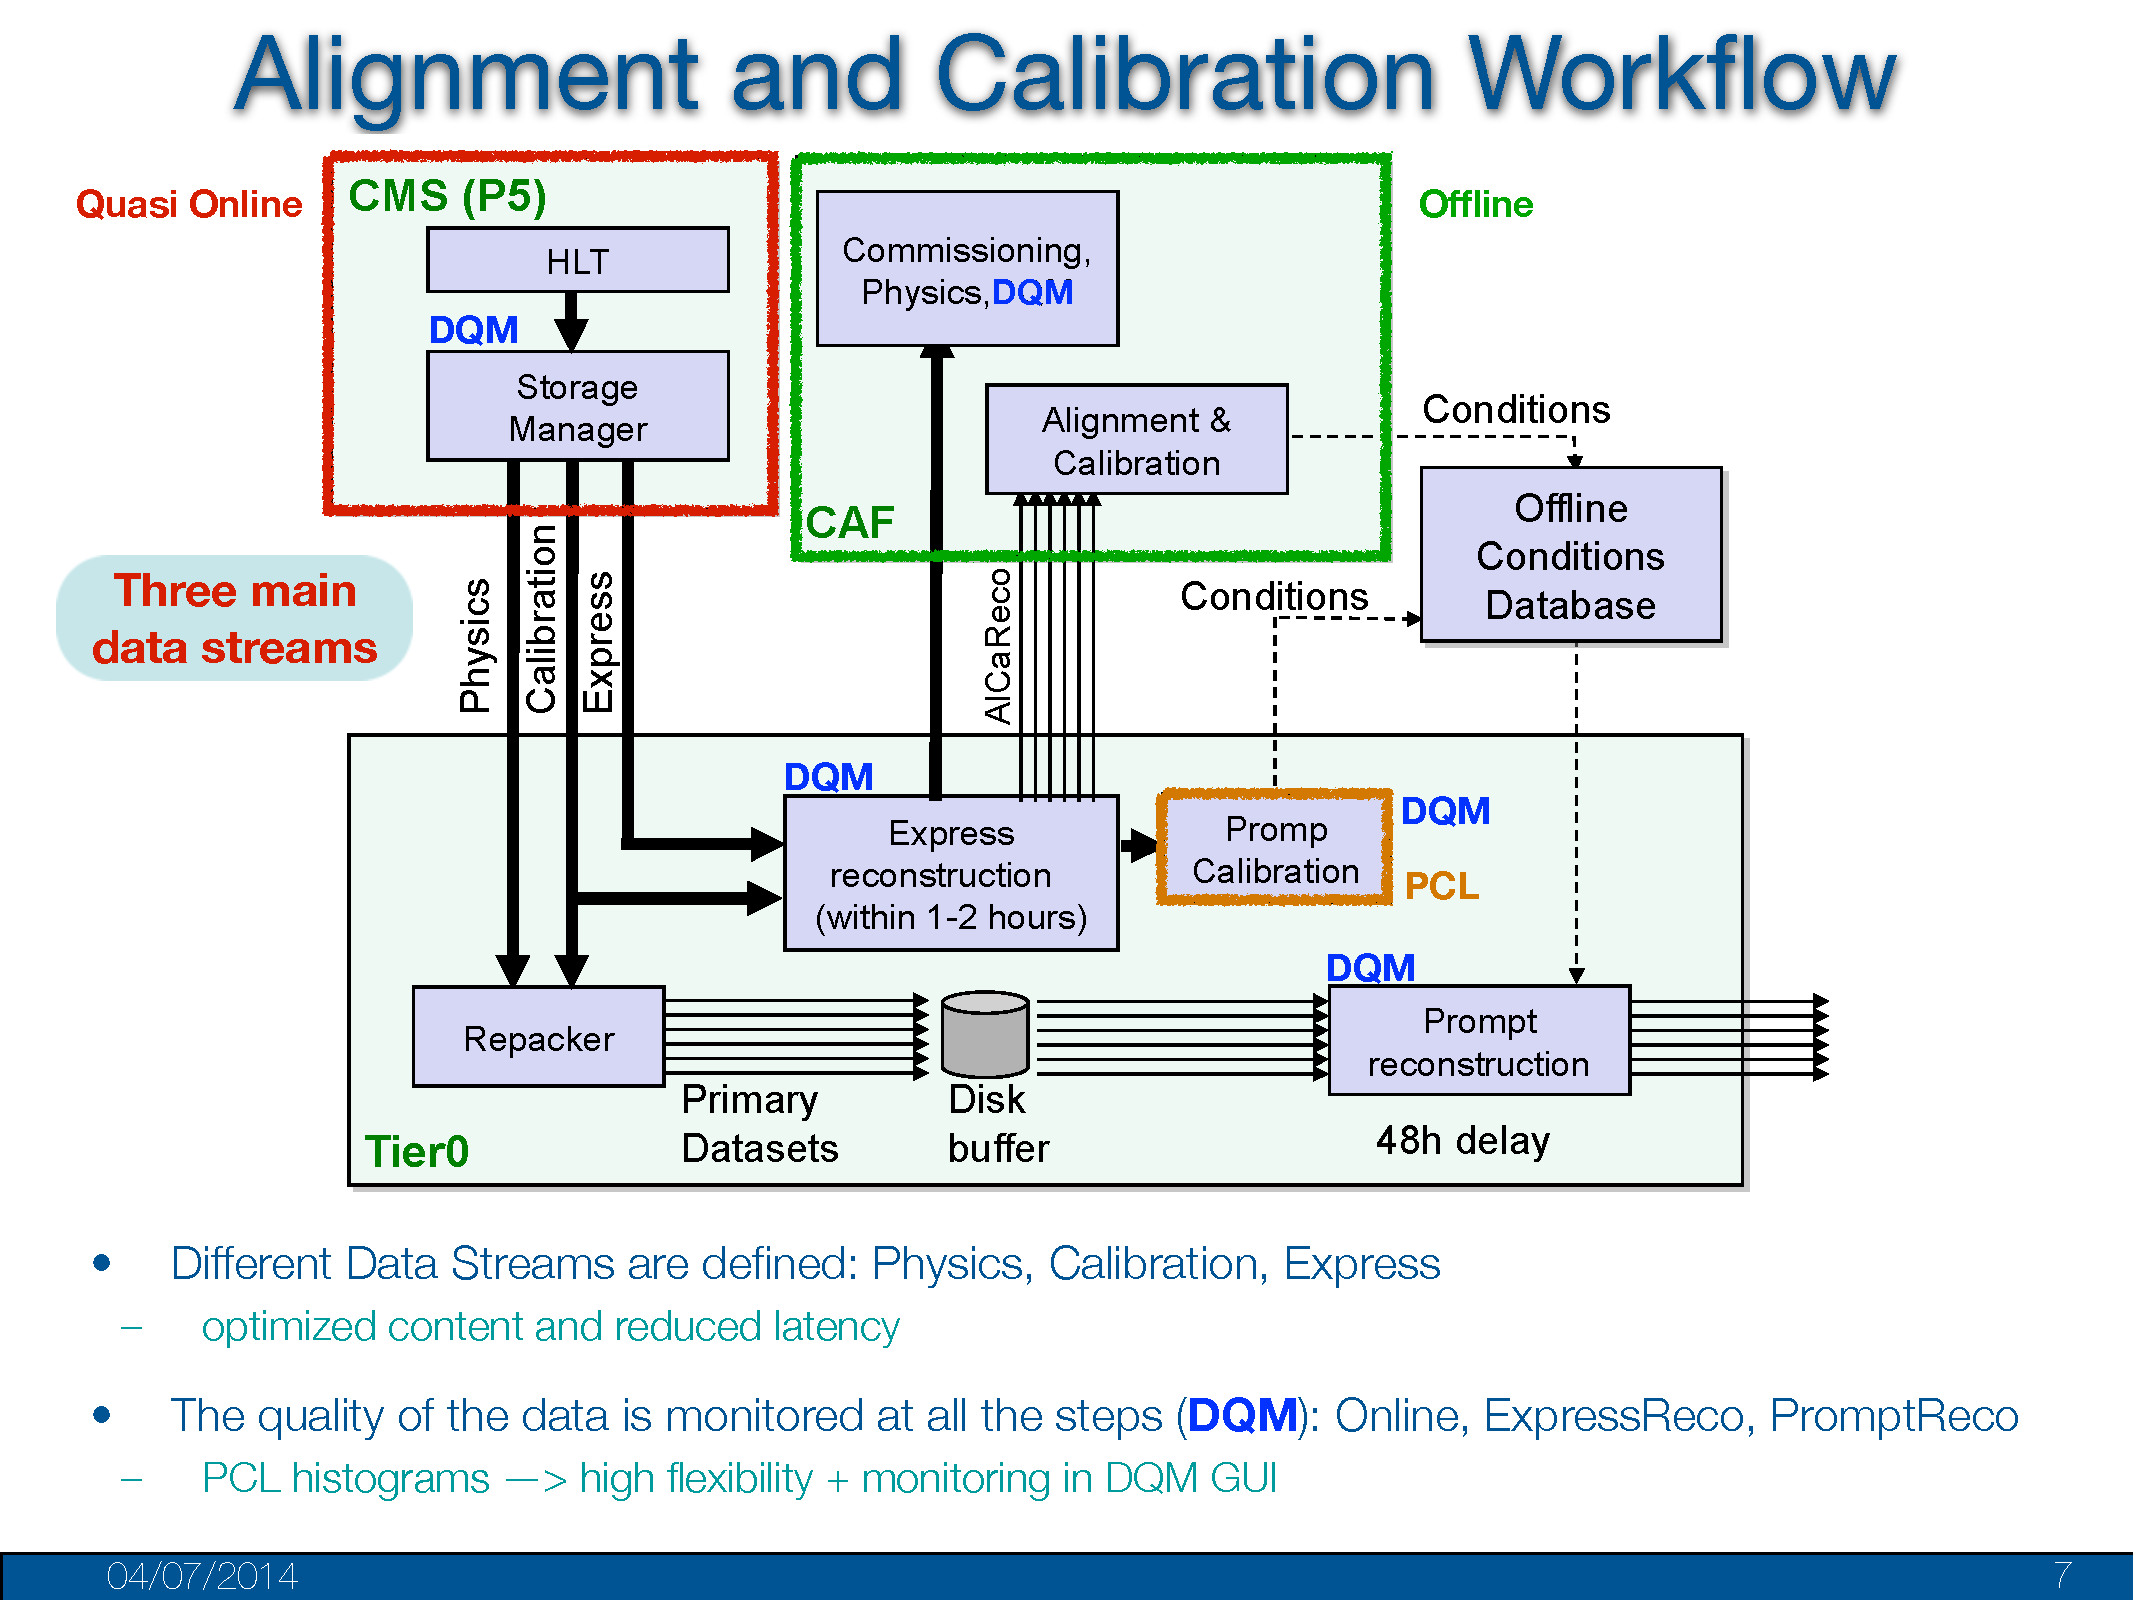
\includegraphics[width=.9\textwidth,clip=true,viewport=0 180 900 700]{figs/cms/AlCa.pdf}
\caption{Alignment and calibration data-processing flow.\label{fig:AlCa}}
\end{figure}

